% This is samplepaper.tex, a sample chapter demonstrating the
% LLNCS macro package for Springer Computer Science proceedings;
% Version 2.20 of 2017/10/04
%
\documentclass[runningheads]{llncs}
%
\usepackage{caption}
\usepackage{subcaption}
\usepackage{todonotes}
\usepackage{amsmath}
\usepackage{url}
\usepackage{graphicx}
\usepackage{hyperref}

\newenvironment{MyFigure}[1][]{\begin{figure}[#1]\vspace{-0.5cm}}{\vspace{-0.5cm}\end{figure}}
% Used for displaying a sample figure. If possible, figure files should
% be included in EPS format.
%
% If you use the hyperref package, please uncomment the following line
% to display URLs in blue roman font according to Springer's eBook style:
% \renewcommand\UrlFont{\color{blue}\rmfamily}

\begin{document}
%
\title{Medical Image Analysis Assignment 3}
%
%\titlerunning{Abbreviated paper title}
% If the paper title is too long for the running head, you can set
% an abbreviated paper title here
%
\author{Casper Bresdahl}
%
% \authorrunning{F. Author et al.}
% First names are abbreviated in the running head.
% If there are more than two authors, 'et al.' is used.
%
% \institute{Princeton University, Princeton NJ 08544, USA \and
% Springer Heidelberg, Tiergartenstr. 17, 69121 Heidelberg, Germany
% \email{lncs@springer.com}\\
% \url{http://www.springer.com/gp/computer-science/lncs} \and
% ABC Institute, Rupert-Karls-University Heidelberg, Heidelberg, Germany\\
% \email{\{abc,lncs\}@uni-heidelberg.de}}
%
\maketitle              % typeset the header of the contribution
%
\section{Introduction}
This week we will first introduce the theory behind advection and mean curvature flow and how we can discretize these. We will then look at the first experiment looking into how advection without any boundary issues behave compared to advection where boundaries will play a role. We will then look at the second experiment where we will compare three different boundary conditions and how these change the end result when applying mean curvature flow to a signed distance field. At the end we will conclude on our results.
\section{Image registration}
Image registration is the problem of aligning two similar images such that their main features overlap. Applications of image registration ranges from two images of the 'real world' taken of the same scene with slightly different angles, to when an x-ray and an MRI scan, both sharing similar modalities, needs to be aligned or when the results of a treatment needs to be compared based on a follow up scan, to when an MRI scan, which shows structure, needs to be aligned with a PET scan, which could show tumor growth, where these scans do not share the same modality. Similar for all applications we would like to perform a transformation on one image, which gives us the same image, but seen in the perspective / space of the other, such that the two images becomes the most similar.
\section{Similarity}
The image registration problem can be written as an optimization problem where we would like to maximize / minimize some measure of similarity. To name a few similarity measures we have \textit{sum of squared differences} (SSD), \textit{generalized p-norm}, \textit{normalized cross correlation} (NCC), \textit{mutual information} (MI) and \textit{normalized mutual information} (NMI). The first two needs to be minimized as they describe the distance between two compared pixels, whereas the rest needs to be maximized. All similarity measures play the same role in the optimization problem, to measure the similarity between the two images. Which similarity measure to use depends on the task at hand. Because SSD, P-norm and NCC uses pixel intensities to compute the similarities they are not intensity invariant, and so, they can not measure similarity between images of different modalities. On the other hand, MI and NMI uses distributions to compute the similarities, and so, as long as the distribution of pixel intensities stays the same, it does not matter which intensity they have, and so MI and NMI are intensity invariant and can be used to compare images of different modalities. This means the similarity measure we choose plays a role in which types of images we can compare. On the flip side, SSD is a very simple quadratic function, and we would expect this to be much easier and faster to optimize than the more complex NMI, and so the similarity measure we choose also has a role in the speed of our registration.
\section{Regularization}
Regularization is used as extra terms in the optimization problem to penalize unwanted behaviour. If we simply optimize without regularization it might be we get a decent transformation at all points except one, where it lies very far away from where we would expect. In that scenario we can add a regularization term which takes the difference in \textit{x} and \textit{y} coordinates before and after the transformation and squares this distance and adds it or subtracts it (depending on our optimization problem) from our optimization to penalize single major errors. This effectively makes the algorithm prefer many small errors in our transformation rather than few major errors. Another example of a regularization term could be to penalize folding as a solution to minimize distances. This can be done by adding a regularization terms which add / subtracts from our optimization depending on the sign of the transformation. Many more regularizations exists, and as long as they add or subtract from the optimization they can be used as regularization terms. Of course it is possible to over regularize an optimization, in which case the optimal solution might simply become to not do any transformation as this is less punishing than transforming the image, and so, one must be careful not to make the optimization too restrictive.
\section{Different types of transformations}
There exists different types of transformations which can be performed on images, three of them are \textit{rigid}, \textit{affine} and \textit{non-rigid}. A rigid transformation describes a rotation, an \textit{x} translation and a \textit{y} translation. This means the image can be moved a number of pixels in the \textit{x} and \textit{y} direction along being rotated. This is the simplest transformation, but given it only consists of three parameters it is also the easiest to optimize. The transformation matrix used to describe a rigid transformation would be:
\begin{equation*}
	\begin{bmatrix}
		cos(\theta) & -sin(\theta) & t_x \\
		sin(\theta)  &  cos(\theta) & t_y \\
		0				 & 0				 & 1
	\end{bmatrix}
\end{equation*}
The transformations it can make can be visualized as the top row of \autoref{rigidAffine}. A combination of translation and rotation can also be made.

\begin{figure}[h]
	\centering
	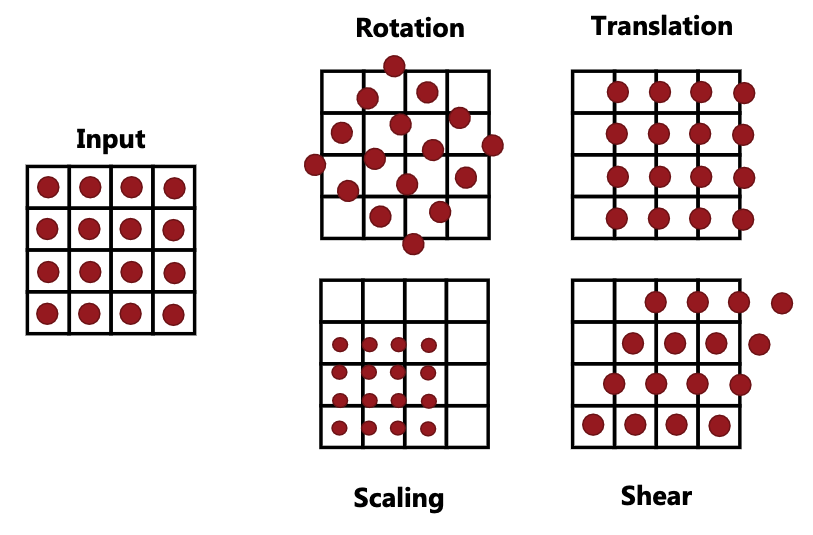
\includegraphics[width=0.75\linewidth]{Materials/affineRigid}
	\caption{Input image along a row of rigid transformations (top) and a row of affine transformations (bottom). Image taken from lecture slides.}
	\label{rigidAffine}
\end{figure}
An affine transformation can in addition to translations and rotations make scaling and shearing effects. Because of this, it requires additional parameters to optimize. The transformation matrix can be written as:
\begin{equation*}
	\begin{bmatrix}
		1+p_1 & p_2 & p_3\\
		p_4  &  1+p_5 & p_6\\
		0				 & 0				 & 1
	\end{bmatrix}
\end{equation*}
The plus 1 are used to ensure we find the identity matrix if the optimal solution is to apply no deformation. The transformations it can make can be seen in \autoref{rigidAffine} where the bottom row is affine transformations. A combination of all aforementioned transformations can also be made.\\
A non-rigid transformation has even more parameters, but can again perform even greater deformations to the image, like circular, curved, arbitrary and stretched transformations. As it has nine parameters it is the hardest of the three transformations to find an optimal solution for. The transformation matrix can be written as:
\begin{equation*}
	\begin{bmatrix}
		1+p_1 & p_2 & p_3\\
		p_4  &  1+p_5 & p_6\\
		p_7	 & p_8	& 1+p_9
	\end{bmatrix}
\end{equation*}
The transformations it can make can be seen in \autoref{nonrigid}. Along these new transformations it can also perform rigid and affine transformations and any combination of the specific transformations. 

\begin{figure}[h]
	\centering
	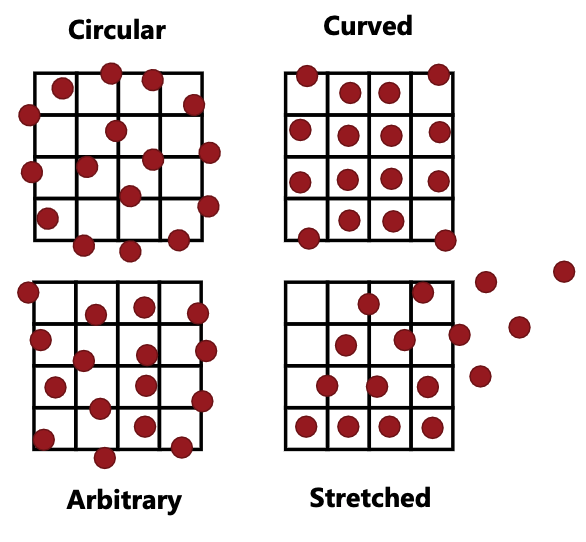
\includegraphics[width=0.55\linewidth]{Materials/noneRigid}
	\caption{Examples of non-rigid transformations. Image taken from lecture slides.}
	\label{nonrigid}
\end{figure}
As the complexity of optimization increases with each additional parameter which needs to be optimized, we use each type of transformations in different contexts. As a rigid transformation can not deform the image, it is often chosen when we have intra-subject images where we expect the scanned object to keep its shape. This could be intra-subject brain MRI, perhaps a follow up scan, as we do not expect the patient's brain to change in shape or size, but we do expect the patient to lie differently in the MRI scanner at each scan. Affine transformations are often chosen when we compare inter-subject images. Here we might want to compare an ill brain to a healthy one, and so we expect small scale differences or small variations in shape. Non-rigid transformations are used when we want to compare object which potentially can have very different shapes. This could be intra- or inter-subject lung CT scans where the patient is breathing while the scan is performed and thus two intra-subject scans might end up very differently. In addition, the shapes of lungs greatly varies between patients, and so strong deformation might be needed to align two lung CT scans.
\section{Non-rigid registration}
We can now perform a non-rigid transformation of two lung pairs in python. In \autoref{registration} we see the two images used along the results of the registration using MI and NCC. The male lungs have been chosen as the moving image for both registrations and the female lungs as the fixed image. This means the male lungs are transformed to match the female lungs. 

\begin{figure}[h]
	\centering
	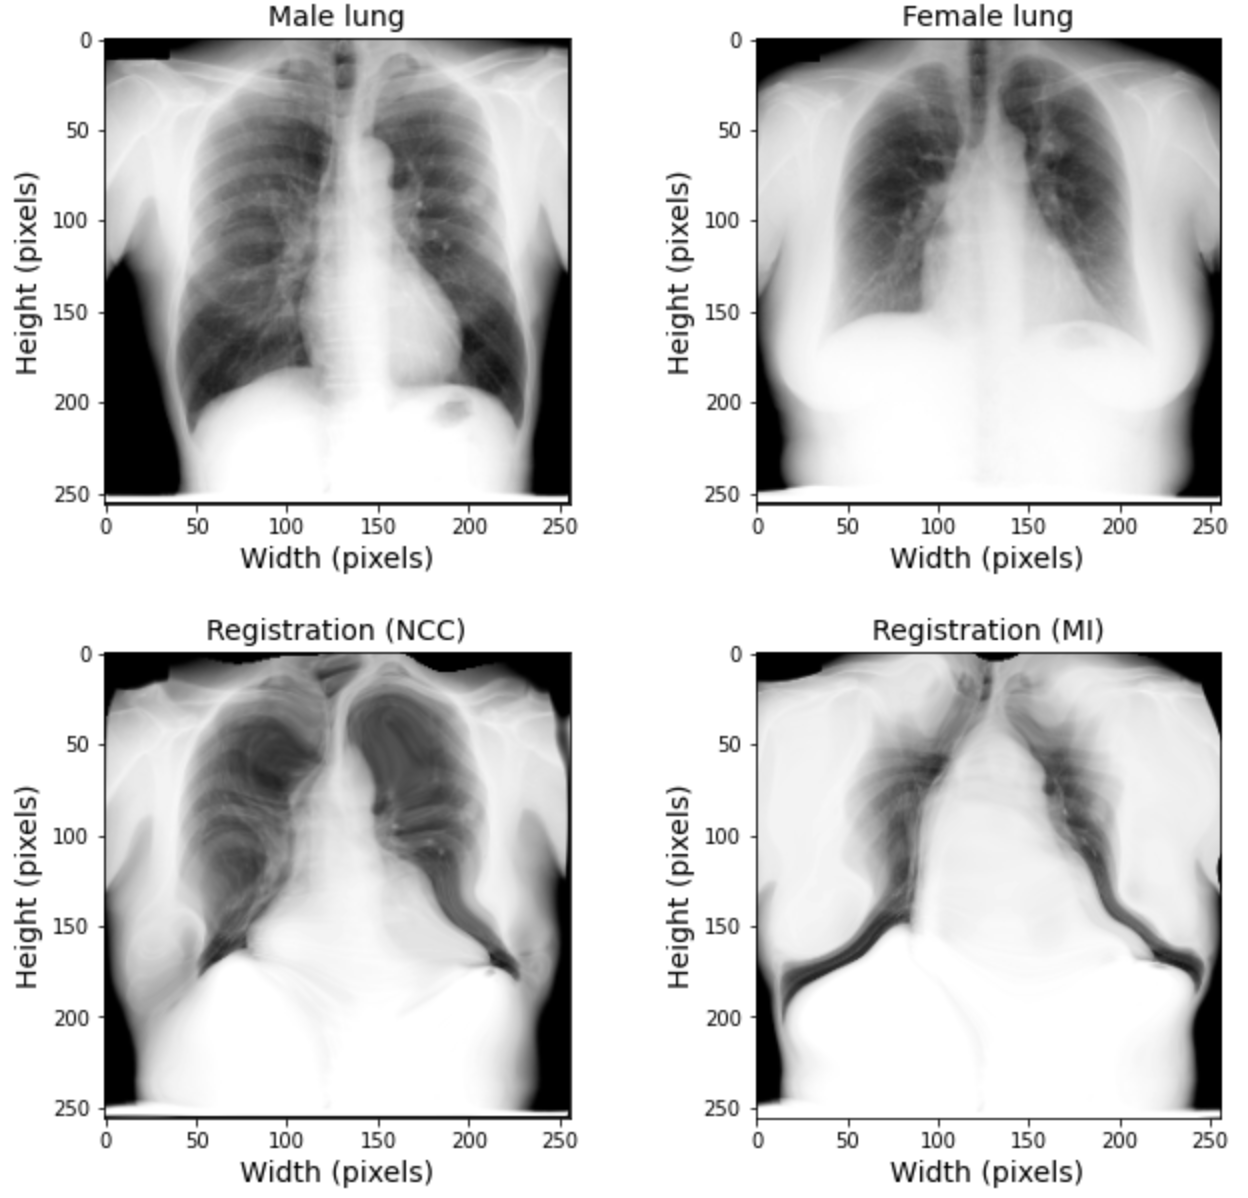
\includegraphics[width=0.8\linewidth]{Materials/registration}
	\caption{Top left: male lungs which will get registered to the female lungs. Top right: female lungs. Bottom left: result of registration performed with NCC. Bottom right: Result of registration performed with MI.}
	\label{registration}
\end{figure}
As seen, the registration using NCC captures that the male lungs needs to be squished and scaled down to match the female lungs, and the top part of both lungs seems to match the female lungs quite well. However, the lower part becomes very deformed and unrealistic. The ribs which previously were slightly curved but otherwise even are now completely curved which does not match the female lungs. Overall the registration has become quite unrealistic, but the images we register are also \textit{very} different. Looking at the MI results, we see the lungs have almost completely collapsed. This is likely due to the fact that MI is measured based on the distribution of pixel intensities, and because the distribution in the two images is so different, optimization based on MI becomes very difficult, and a local maxima is found instead. As NCC uses the intensities directly rather than their distribution we see it is much easier to optimize with NCC. This illustrates the importance of using the correct Similarity measure for the task at hand.
\section{Conclusion}
In conclusion we have seen where segmentation can be used in medical image analysis, we have seen the risks of dilation and erosion and explained the benefits of them, we have concluded Graph cut segmentations are preferred, but also have limited applications and Random walker alleviates these constrains by being non-deterministic, and finally we have looked into how PCA can be used for segmentation.
\newpage
%
% ---- Bibliography ----
%
% BibTeX users should specify bibliography style 'splncs04'.
% References will then be sorted and formatted in the correct style.
%
% \bibliographystyle{splncs04}
% \bibliography{mybibliography}
%
%\begin{thebibliography}{8}
%\bibitem{MIA}
%A.P. Dhawan, Medical Image Analysis, 2nd edition, 2011, John Wiley
%
%\bibitem{MIS}
%A. Maier, et al., Medical Imaging Systems, 2018, Springer Open
%
%\end{thebibliography}
\section{Code collaboration}
The code for this assignment has been developed in collaboration with Marcus Hansen, Sarah Hansen and Ulrik Larsen.
\end{document}
